\chapter{Applicazione Mobile}

In questo capitolo verrà presentato un esempio di applicazione mobile in grado di connettersi al \emph{City Service} e di eseguire le operazione di prenotazione e ritiro delle ricariche. Il suo scopo è permettere all'utente di eseguire operazioni di interazioni con la smart-city al fine di ridurre le problematiche derivanti dall'utilizzo di veicoli elettrici. In particolare permette di eseguire richieste e cancellazioni di prenotazioni di ricariche attraverso i protocolli visti nella sezione ~\ref{sec:protocol}.

Inizialmente si limitava solo a queste operazioni ovvero prenotazione e cancellazioni di ricariche e inoltre funzionava solo in presenza del simulatore (~\ref{chap:sim}) in quanto prendeva il possesso di un veicolo gestito dal simulatore stesso. Il funzionamento è stato poi ampliato con la possibilità di connettersi tramite \emph{Bluetooth} a un veicolo reale, opportunità concessa dal \emph{Centro Ricerche Fiat} (\emph{CRF}), oppure di connettersi in assenza di veicoli.

A questo si è aggiunta la possibilità di analizzare il profilo altimetrico che separa il dispositivo mobile da un determinato EVSE con lo scopo di fare previsioni più accurate sui consumi necessari a raggiungerlo.

La piattaforma di sviluppo scelta è \emph{Android} vista la sua grandissima diffusione e versatilità.

\section{Architettura}

La piattaforma scelta per lo sviluppo è Android dalla versione \emph{4.0.3} in su. Questo perché vanta maggiori performance e un interfaccia utente più bella è più facile da programmare. La libreria di base per interfacciarsi con il SIB è quella esposta nella sezione ~\ref{subsec:ioe-lib}.

\subsection{Interazione con L'esterno}

L'interazione con il servizio cittadino avviene tramite scambio di messaggi con il \emph{City SIB}, mentre le informazioni relative al veicolo, in particolar modo se quest'ultimo è simulato, arrivano dal \emph{Dash SIB}.


\section{Modalità di esecuzione}

L'applicazione al fine di adattarsi ai diversi scenari possibili offre molteplici modalità di esecuzione, questo per adattarsi alle specifiche richieste per le dimostrazioni del Remote ??Monitoring¿¿. La scelta della modalità di esecuzione avviene nella schermata iniziale come si può vedere in figura ~\ref{fig:main-activity}

\subsection{Simulazione}

Questa modalità permette di prendere il controllo di un veicolo contenuto nel simulatore, il quale deve essere avviato con appositi parametri che causino la scrittura dei parametri relativi ai veicoli sul \emph{Dash SIB}. Questo implica che una volta che i abbiamo premuto sul pulsante \emph{Connect} (Fig. ~\ref{fig:main-activity}), dobbiamo scegliere l'utente Luciano Bononi in quanto è l'utente di default usato dalle macchine del simulatore (Fig. ~\ref{fig:select-user}). Una volta selezionato l'utente ci troveremo nel menu principale con solo due opzioni (Fig. ~\ref{fig:main-menu}). Questo perché le altre opzioni sono subordinate alla scelta di un veicolo. Una volta selezionato il veicolo (Fig. ~\ref{fig:select-veh}) vedremo esattamente i parametri che esso ha nel simulatore (posizione, carica, potenza ecc..). La posizione segnata nella mappa dell'app sarà la stessa segnata su SUMO. L'interazione tra il veicolo 

\begin{figure}[H]
        \centering
        \begin{subfigure}[H]{0.3\textwidth}
                \adjincludegraphics[width=\textwidth,trim={0 {0.5\height} 0 0},clip]{assets/mobile-app-select-user.png}
                \caption{Selezione Utente.}
                \label{fig:select-user}
        \end{subfigure}%
        ~ %add desired spacing between images, e. g. ~, \quad, \qquad etc.
          %(or a blank line to force the subfigure onto a new line)
        \begin{subfigure}[H]{0.3\textwidth}
                \adjincludegraphics[width=\textwidth,trim={0 {0.5\height} 0 0},clip]{assets/mobile-app-main-menu.png}
                \caption{Menu principale senza nessun veicolo selezionato}
                \label{fig:main-menu}
        \end{subfigure}
        \begin{subfigure}[H]{0.3\textwidth}
                \adjincludegraphics[width=\textwidth,trim={0 {0.5\height} 0 0},clip]{assets/mobile-app-select-veh.png}
                \caption{Selezione veicolo}
                \label{fig:select-veh}
        \end{subfigure}
        \caption{Schermate Applicazione Mobile}
\end{figure}

\subsection{Con Blue Me}

\subsection{Senza Blue Me}


\begin{figure}
	\centering
	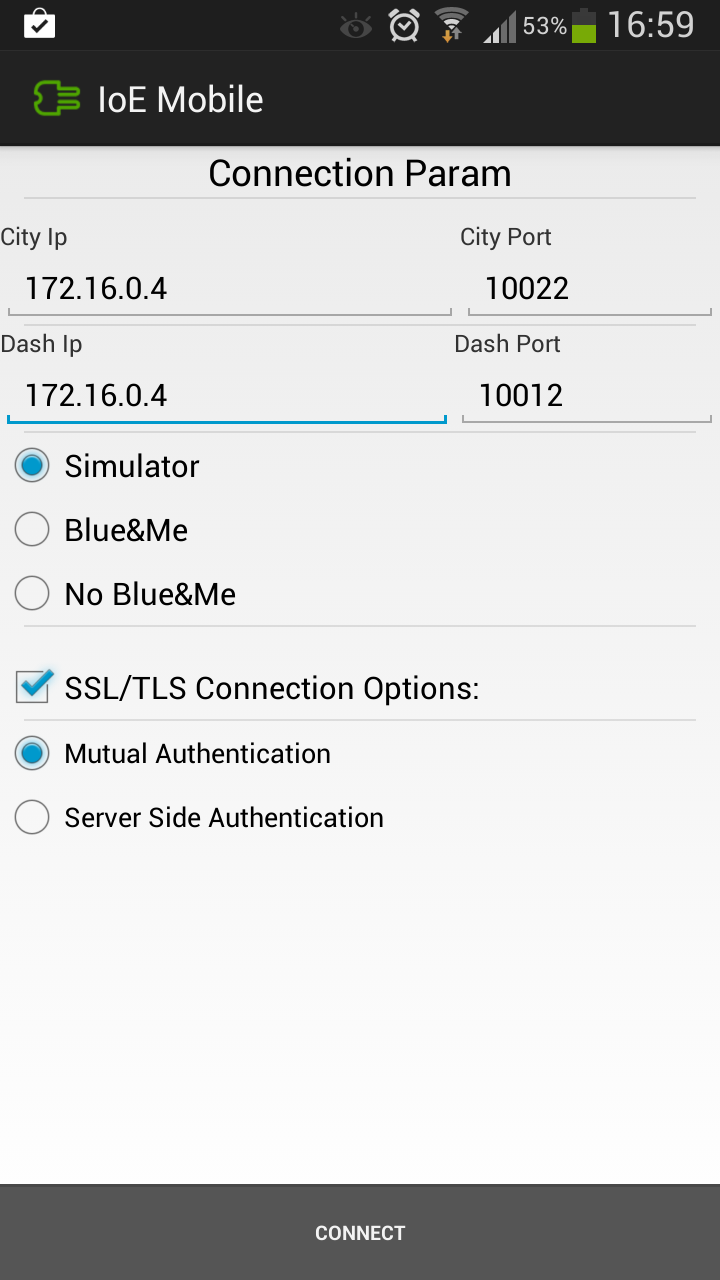
\includegraphics[width=0.3\textwidth]{assets/mobile-app-main.png}
	\caption{Schermata Principale con i parametri di connessione ai SIB e la scelta di modalità di esecuzione.}
	\label{fig:main-activity}
\end{figure}


\section{Richiesta di prenotazione}

\section{Activities}
